% Options for packages loaded elsewhere
\PassOptionsToPackage{unicode}{hyperref}
\PassOptionsToPackage{hyphens}{url}
%
\documentclass[
]{article}
\usepackage{lmodern}
\usepackage{amssymb,amsmath}
\usepackage{ifxetex,ifluatex}
\ifnum 0\ifxetex 1\fi\ifluatex 1\fi=0 % if pdftex
  \usepackage[T1]{fontenc}
  \usepackage[utf8]{inputenc}
  \usepackage{textcomp} % provide euro and other symbols
\else % if luatex or xetex
  \usepackage{unicode-math}
  \defaultfontfeatures{Scale=MatchLowercase}
  \defaultfontfeatures[\rmfamily]{Ligatures=TeX,Scale=1}
\fi
% Use upquote if available, for straight quotes in verbatim environments
\IfFileExists{upquote.sty}{\usepackage{upquote}}{}
\IfFileExists{microtype.sty}{% use microtype if available
  \usepackage[]{microtype}
  \UseMicrotypeSet[protrusion]{basicmath} % disable protrusion for tt fonts
}{}
\makeatletter
\@ifundefined{KOMAClassName}{% if non-KOMA class
  \IfFileExists{parskip.sty}{%
    \usepackage{parskip}
  }{% else
    \setlength{\parindent}{0pt}
    \setlength{\parskip}{6pt plus 2pt minus 1pt}}
}{% if KOMA class
  \KOMAoptions{parskip=half}}
\makeatother
\usepackage{xcolor}
\IfFileExists{xurl.sty}{\usepackage{xurl}}{} % add URL line breaks if available
\IfFileExists{bookmark.sty}{\usepackage{bookmark}}{\usepackage{hyperref}}
\hypersetup{
  pdftitle={Desire to learn about the benefits of medical cannabis for chronic pain?},
  pdfauthor={Jeya Seenivasagam, James Wall, and Surya Gutta},
  hidelinks,
  pdfcreator={LaTeX via pandoc}}
\urlstyle{same} % disable monospaced font for URLs
\usepackage[margin=1in]{geometry}
\usepackage{longtable,booktabs}
% Correct order of tables after \paragraph or \subparagraph
\usepackage{etoolbox}
\makeatletter
\patchcmd\longtable{\par}{\if@noskipsec\mbox{}\fi\par}{}{}
\makeatother
% Allow footnotes in longtable head/foot
\IfFileExists{footnotehyper.sty}{\usepackage{footnotehyper}}{\usepackage{footnote}}
\makesavenoteenv{longtable}
\usepackage{graphicx,grffile}
\makeatletter
\def\maxwidth{\ifdim\Gin@nat@width>\linewidth\linewidth\else\Gin@nat@width\fi}
\def\maxheight{\ifdim\Gin@nat@height>\textheight\textheight\else\Gin@nat@height\fi}
\makeatother
% Scale images if necessary, so that they will not overflow the page
% margins by default, and it is still possible to overwrite the defaults
% using explicit options in \includegraphics[width, height, ...]{}
\setkeys{Gin}{width=\maxwidth,height=\maxheight,keepaspectratio}
% Set default figure placement to htbp
\makeatletter
\def\fps@figure{htbp}
\makeatother
\setlength{\emergencystretch}{3em} % prevent overfull lines
\providecommand{\tightlist}{%
  \setlength{\itemsep}{0pt}\setlength{\parskip}{0pt}}
\setcounter{secnumdepth}{5}
\usepackage{fancyhdr}
\pagestyle{fancy}
\fancyhead[LO,LE]{}
\fancyhead[RO,RE]{Medical Cannabis Experiment - Section 1 (Fall 2020)}
\fancyfoot[LO,LE]{Jeya, James, and Surya}
\fancyfoot[CO,CE]{}
\fancyfoot[RE,RO]{\thepage}
\renewcommand{\headrulewidth}{0.5pt}
\renewcommand{\footrulewidth}{0.5pt}

\title{\textbf{Desire to learn about the benefits of medical cannabis for
chronic pain?}}
\author{\textbf{\emph{Jeya Seenivasagam, James Wall, and Surya Gutta}}}
\date{\emph{W241 Experiment - Section 1 (Fall 2020)}}

\begin{document}
\maketitle

{
\setcounter{tocdepth}{2}
\tableofcontents
}
\pagebreak

\begin{center}
Abstract
\end{center}
\begin{center}
TODO - this will have to come last, after the results are in
\end{center}

\hypertarget{background}{%
\section{Background}\label{background}}

Did you know that September is Pain Awareness month?\(^{[1]}\). Pain is
regarded as chronic when it lasts or recurs for more than 6 months.
According to the Centers for Disease Control and Prevention
(CDC)\(^{[2]}\), in 2016, approximately 20\% of U.S. adults experienced
chronic pain (approximately 50 million individuals) and 8\% of U.S.
adults (approximately 20 million individuals) experienced high-impact
chronic pain. In addition causing literal pain, the CDC\(^{[2]}\)
estimates that chronic pain also costs Americans at least 560 billion
USD per year in medical expenses, lost productivity, and disability
programs. Chronic pain can additionally lead to mental health issues,
including anxiety and depression.

The U.S. Department of Health and Human Services (HHS)\(^{[3]}\) has a
developmental objective to ``decrease the prevalence of adults having
high-impact chronic pain''. According to the HHS, treatment for chronic
pain usually focuses not on curing the pain but on managing it -
reducing the pain and increasing people's ability to move and function
so their day-to-day life can improve. Treatment options include
prescription pain medications, acupuncture, physical therapy, relaxation
techniques, biofeedback, massage therapy, psychotherapy, and behavior
modification.

In the United States, individuals who suffer from pain are often
prescribed opioids\(^{[4]}\) to treat their conditions. Over-dependence
on opioids has contributed to what has been dubbed as an `opioid crisis'
in the U.S. The dangers of prescription misuse, opioid use disorder, and
overdose have been a growing problem throughout the U.S. From 1999 to
2018, more than 232,000 people died in the U.S. from overdoses involving
prescription opioids. Overdose deaths involving prescription opioids
were more than four times higher in 2018 than in 1999, according to
CDC\(^{[5]}\). Even as the amount of opioids prescribed and sold for
pain has increased, the amount of pain that Americans report has not
similarly changed. At present, this is almost a disproportionately
American problem - the U.S. constitutes less than 5 percent of the
world's population yet consumes 80 percent of the world's opioid supply.

Doctors now struggle to balance caring for patients with debilitating
pain and meeting new standards and guidelines for opioid prescriptions.
It is clear that opioids cannot be the end solution for chronic pain due
the ongoing opioid crisis in the United States. Solving the `chronic
pain problem' represents a lucrative opportunity. Consequently,
researchers have begun to explore alternatives to opioids, such as
medical marijuana.

According to the National Institutes of Health's National Center for
Complementary and Integrative Health\(^{[6]}\), medical marijuana, also
known as cannabis, has been used in medical treatment for more than
3,000 years for a plethora of conditions, including pain relief,
digestive issues, and psychological disorders. Some studies have
concluded that medical cannabis may be a viable alternative for
opioids\(^{[7]}\).

\hypertarget{research-question}{%
\section{Research Question}\label{research-question}}

It is estimated that 2.1 million Americans (approximately 0.64\% of U.S.
adults) use medical cannabis, whereas approximately 50 million Americans
(approximately 20\% of U.S. adults) have chronic pain. The World Health
Organization (WHO) reports that an estimated 147 million people, 2.5\%
of the world population, consume cannabis annually\(^{[8]}\). The
disparities between these numbers demonstrate the opportunity for
medical cannabis as a painkiller.

In the U.S., the use of cannabis for medical purposes is legal in 33
states (as of before the 2020 election, when several additional states
voted to legalize cannabis for medical purposes), four out of five
permanently inhabited U.S. territories, and the District of
Columbia\(^{[9]}\).

The chemistry of cannabis is anything but straightforward, and its
complexity has made it difficult to discern long and short-term effects
on participants. Consequently it is difficult to easily write a
digestible FAQ on the benefits and risks of the substance. Furthermore,
cannabis is generally considered to be a political subject in the United
States. As a result of its politicized nature, there are a lot of
Americans writing and sharing opinions about cannabis that do not
necessarily rely on data or scientific analysis. This onslaught of
non-scientific information on the subject has lead to copious amounts of
misinformation on the use of marijuana getting spread to the American
population. As people are dying in the U.S. from overdoses involving
prescription opioids, can we educate people suffering from chronic pain
about the benefits of medical cannabis? If yes, will they opt for
medical cannabis?

Our research question is, \textbf{\emph{`Does providing some info on the
benefits of medical cannabis for chronic pain increase participants'
desire to learn more?'}}

\hypertarget{prior-beliefs}{%
\section{Prior Beliefs}\label{prior-beliefs}}

The following beliefs will be validated with the experiment:\\
1. US residents are interested in learning more about the medical
benefits of cannabis if they know its benefits as the opioids deaths are
increasing.\\
2. Cannabis is portrayed as more harmful than it actually is.\\
3. There is a lot of misinformation about medical cannabis.\\
4. US residents believe that Medical cannabis is addictive.

\hypertarget{research-design}{%
\section{Research Design}\label{research-design}}

\hypertarget{idealized-experimental-design}{%
\subsection{Idealized experimental
design}\label{idealized-experimental-design}}

Since chronic pain is a global issue, our idealized experiment would
include participants living across the globe. We would only select
participants who experience chronic pain and who live in states or
countries where medical marijuana is legal. Ideally, more than a million
participants would be recruited to increase the experiment's accuracy
and to ensure the results could be attributed globally. Participants on
pain medication and not on medical cannabis could be recruited through
social media ads and print media advertisements. During the experiment
execution phase, participants will be given one-on-one sessions at their
homes on medical cannabis benefits. We would also like to evaluate the
treatment participants' level of knowledge on cannabis by giving a
simple exam before and after the treatment. One-on-one sessions are
better as many people globally don't have access to the internet or use
technology.

A further optimization to this idealized experiment could involve a
natural experiment, in which the researchers put up a control
advertisement in certain cities and a treatment experiment in other
cities. The researchers could then observe participants interacting with
the advertisements and measure the corresponding effects. This would
also allow us to cluster our participants based on physical location. We
believe that this idealized natural experiment would have the same
properties as a true, controlled experiment.

An alternative route would be to examine cannabis and opiate-related
advertisements in states where cannabis is legal versus those in states
where cannabis is not legal. This would allow the researchers to get
observational data clustered by city and infer a reasonable conclusion
based on this data.

\hypertarget{non-idealized-realistic-design-given-constraints}{%
\subsection{Non-idealized, realistic design given
constraints}\label{non-idealized-realistic-design-given-constraints}}

The idealized experimental design involves more time and money than the
researchers have available to them. As a result, the authors of this
paper will narrow the scope of the experimental design to accommodate
our time and money limitations. We will narrow the scope of our
participants to only U.S. participants. We will accept participants from
all states and who are experience all levels of pain (including none at
all) and will treat location and pain-level as covariates.

Due to the ongoing COVID-19 pandemic, we are unable to conduct our
surveys in person. Consequently, we will conduct our research in an
online setting - participants will be recruited through Amazon MTurk and
will complete a survey through Qualtrics.

\hypertarget{hypotheses}{%
\subsection{Hypotheses}\label{hypotheses}}

\textbf{Primary Outcome}\\
\emph{Desire to learn more about medical cannabis}\\
\(H_{0}\): \emph{There is no desire to learn more about medical
cannabis's benefits for chronic pain after providing some info on
medical cannabis benefits.}

\(H_{a}\): \emph{There is a desire to learn more about medical
cannabis's benefits for chronic pain after providing some info on
medical cannabis benefits.}

\textbf{Other Outcomes}

\emph{Medical cannabis is generally portrayed as more harmful than it
actually is}\\
\(H_{0}\): \emph{Cannabis is not portrayed as more harmful than it
actually is.}

\(H_{a}\): \emph{Cannabis is portrayed as more harmful than it actually
is.}

\emph{Lot of misinformation about medical cannabis}\\
\(H_{0}\): \emph{There is no misinformation about medical cannabis.}

\(H_{a}\): \emph{There is misinformation about medical cannabis.}

\emph{Medical cannabis is addictive}\\
\(H_{0}\): \emph{Medical cannabis is not addictive.}

\(H_{a}\): \emph{Medical cannabis is addictive.}

\hypertarget{analytic-plan}{%
\subsection{Analytic Plan}\label{analytic-plan}}

The following is our analytic plan:\\
1. Analyze the distribution of outcome measures.\\
2. Estimate the effect(s) using regression after controlling for a set
of covariates.\\
3. Compute robust standard errors.\\
4. Compute heterogeneous treatment effects.

\hypertarget{participants}{%
\subsection{Participants}\label{participants}}

\textbf{How participants are recruited}

The opioid epidemic is by far the most prevalent in the U.S..
Consequently, we believe it is acceptable to limit this experiment to
American participants (around 250\textasciitilde500 participants). Since
there is a risk of non-homogeneity of participants that we may get
through social media, participants will be recruited using Amazon
Mechanical Turk (MTurk)\(^{[10]}\).

After a subject from MTurk starts the survey, that subject is randomly
assigned to either the placebo or the treatment group. We are able to
achieve complete randomization by employing Qualtrics' survey technology
to completely and blindly assign participants to one group. We recognize
that often times deliberate variation within subgroups via an
intervention can sometimes be more useful in terms of observing a
treatment effect than pure randomization. Having said that, in this
specific case we felt that complete randomization of participants within
age blocks (as detailed later in this paper) is more appropriate for
this specific experiment. We believe this is the case because we did not
want to further divide participants based on other subject attributes
(e.g.~gender, ethnicity) and potentially introduce bias from the
experimenters' preconceived notions. Complete randomization within age
blocks allows us to be confident that our experimental results are
representative of American adults.

\textbf{Location of participants}

The legalization status of marijuana varies from U.S. state to U.S.
state. Additionally, recent elections have also affected the
legalization of cannabis in different states. Each U.S. state falls into
one of the following categories: (Marijuana is completely illegal, Only
medical marijuana is legal, Recreational and medical marijuana are
legal, Medical marijuana is not yet legal but was legalized in the 2020
election, Recreational marijuana is not yet legal but was legalized in
the 2020 election). We will collect information on what state an
individual is from and the legal status of marijuana in that state and
consider it as a covariate in this analysis. To make sure that the
non-interference assumption is not violated, we will check the location
of each subject taking the survey using the subject's IP address.

We recognize that we could have considered clustering participants based
on location (clustering on American state). We do not believe that that
this is appropriate for this experiment. Clustering normally comes into
play when it is impossible to randomly assign participants to group
within a given attribute like location. Since we are able to randomly
assign participants to group within location, we choose not to use
clustering in this experimental design.

\textbf{Age of participants}

The legal age for consuming cannabis varies from state to state in the
US. Generally the legal age to consume cannabis is 21 years of age or
older. Consequently, we will not examine participants who are aged less
than 21 years old. MTurk blocks participants at 18-25 and unfortunately
we cannot break this block into the more granular blocks of 18-21 and
21-25. Since we can only ignore the block of participants age 18-25, we
will only allow participants to participate who are at least 25 years
old. We believe it is important to use MTurk's blocks because it helps
us minimize potential \emph{noncompliance issues}, such as the
participants lying about their age so that they can get paid to take the
survey.

Consequently, our experiment uses blocking. We believe that blocking on
age can only be beneficial to experiment. We believe that normally using
MTurk participants would cause an imbalance in subject age, likely
skewing younger as younger participants are more likely to be familiar
with MTurk technology and this employment opportunity. We believe that
blocking on age will allow for more precision by not conducting a
randomization on the age covariate, which we believe would normally be
very imbalanced.

The reader should note that excluding participants that fall within an
age group is common for experiments with small samples. Having said
that, we recognize that this introduces a concern around subject
imbalance. We believe that we are able to maintain an even distribution
across age due to our blocking of age. The consequences of excluding the
youngest age group of adults (age 21-24) is that our participants will
skew older than the overall adult population of the United States. As a
result, this implies that your experimental results may not be valid for
American adults aged 21-24.

Although out the outset it seems that excluding the youngest age group
of American adults might prove to be a detriment to our experiment, we
believe that ignoring the age block of 21-24 is acceptable sine the CDC
reports\(^{[14]}\) that chronic pain is only present in 8.5 percent of
the population for the age group (18-29). We suspect that this number is
even lower for participants aged 21-24.

\hypertarget{block-random-assignment}{%
\subsection{Block Random Assignment}\label{block-random-assignment}}

The participants are blocked by age a)25-35, b)35-45, c)45-55 and d)55
or older. This blocking gives similar potential outcomes as the severity
of the chronic pain varies across age groups and increases the
statistical power. This blocking also reduces sampling variability and
improves the precision of the estimated treatment effect. It will help
us to do further analysis based on age groups. Randomization will be
done within each block, and participants will be assigned to treatment
and placebo groups accordingly.

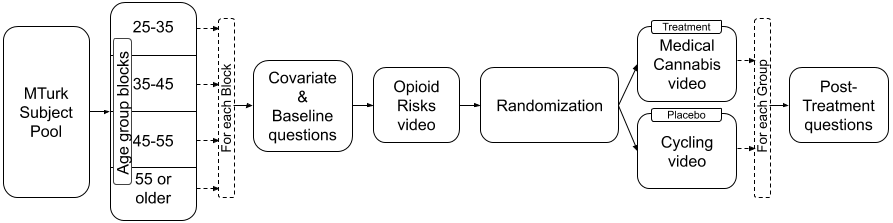
\includegraphics{randomization_chart.png}\\
\hspace*{0.333em}

\hypertarget{treatment}{%
\subsection{Treatment}\label{treatment}}

All the participants will be given an initial questionnaire, generated
by Qualtrics, to get information on the covariates. We will randomize
the participants within the block and assign them to treatment and
placebo groups. Treatment group will be shown videos on Opioids - Risks
\& Side effects and Benefits of Medical Cannabis. Placebo group will be
shown videos on Opioids - Risks \& Side effects and Benefits of Cycling.
In the end, there will be post-treatment five point Likert scale
questions. The experiment duration will be short and the results will be
collected from the Qualtrics service.

\hypertarget{treatment-group-videos}{%
\subparagraph{Treatment group videos}\label{treatment-group-videos}}

\begin{longtable}[]{@{}llll@{}}
\toprule
Video & Title & Link & Duration\tabularnewline
\midrule
\endhead
1 & Opioids - Risks \& Side effects &
\href{https://youtu.be/y0mfzDAs1BE}{{[}Opioids{]}} & 2 min. and 19
sec.\tabularnewline
2 & Benefits of Medical Cannabis &
\href{https://youtu.be/OhJ0YaJXrJo}{{[}Med. Cannabis{]}} & 5 min. and 3
sec.\tabularnewline
\bottomrule
\end{longtable}

\hypertarget{placebo-group-videos}{%
\subparagraph{Placebo group videos}\label{placebo-group-videos}}

\begin{longtable}[]{@{}llll@{}}
\toprule
Video & Title & Link & Duration\tabularnewline
\midrule
\endhead
1 & Opioids - Risks \& Side effects &
\href{https://youtu.be/y0mfzDAs1BE}{{[}Opioids{]}} & 2 min. and 19
sec.\tabularnewline
2 & Benefits of Cycling &
\href{https://youtu.be/xWo0FOwZVX0}{{[}Cycling{]}~~~~~~~~~~} & 5 min.
and 3 sec.\tabularnewline
\bottomrule
\end{longtable}

\hypertarget{assumptions}{%
\subsection{Assumptions}\label{assumptions}}

\textbf{Random Assignment}\\
Randomly assigned the participants to either placebo or treatment groups
within each Age groups by using the same random procedure (Qualtrics
randomizer).

\textbf{Excludability}\\
Excludability restriction is not violated as participants are exposed to
only either placebo or treatment groups. The experiment design ensures
that the same procedures are used to measure outcomes in the placebo or
treatment groups. We strongly believe that no other treatments, research
activities, or third-party interventions occurred during the experiment
as the experiment can be completed in 5 minutes after the random
assignment.

\textbf{Non-Interference (SUTVA)}\\
Care was taken in the experiment's design and execution to avoid
Non-Interference/ Stable Unit Treatment Value Assumption (SUTVA)
violations. We addressed this by a) recruiting the participants
throughout the US so that the participants' interaction is less. We got
186 participants from 41 states. b) Minimized the treatment/placebo
videos time to 5 minutes so that the experiment can be done fast after
the random assignment. The participants discussing over the phone or any
other communication about the experiment is minimized. c) Launched the
experiment on a weekend to avoid participants from the same office so
that they won't discuss with other participants d) If participants are
from the same house, they will have the same IP address, and our program
will flag them as duplicate IP addresses and would be filtered out. We
strongly believe that our experiment upholds the Non-Interference /
Stable Unit Treatment Value Assumption (SUTVA) assumption.

\hypertarget{covariates}{%
\subsection{Covariates}\label{covariates}}

We monitored some of the covariates like Sex (Male/Female/Other),
Race/Ethnicity (American Indian or Alaska Native, Hispanic or Latino,
White, Black or African American, Asian, Native Hawaiian or Other
Pacific Islander, Other), Education (Less than high school, High school,
Some college, Bachelor's degree or higher), Employment status (Employed,
Not employed). We also include an important covariate `Do you experience
chronic pain?'.

\begin{enumerate}
\def\labelenumi{\arabic{enumi}.}
\tightlist
\item
  Gender: Male/Female/Other.
\item
  Age groups: a)25-35, b)35-45, c)45-55 and d)55 or older.
\item
  Ethnic background (White, Black or African American, Hispanic/Latino,
  Asian, Other).
\item
  Education (Less than high school, High school, Some college,
  Bachelor's degree or higher).
\item
  Employment status (Employed, Not Employed).
\item
  State (available from Qualtrics meta information). Note: Using State
  covariate, created another covariate on medical cannabis legality type
  (Legal, Illegal).
\item
  Political beliefs (Liberal, Conservative, Independent/Other).
\end{enumerate}

\textbf{Pre-treatment}(Likert 5 point scale)

\begin{enumerate}
\def\labelenumi{\arabic{enumi}.}
\setcounter{enumi}{7}
\tightlist
\item
  Do you experience chronic pain? (Yes/No)
\end{enumerate}

The following question provides the baseline on the participants
knowledge of prescription opioids and the problems associated with:

\begin{enumerate}
\def\labelenumi{\arabic{enumi}.}
\setcounter{enumi}{8}
\tightlist
\item
  Deaths due to overdoses involving prescription opioids are increasing.
\end{enumerate}

\textbf{Post-treatment Questions}(Likert 5 point scale)

\begin{enumerate}
\def\labelenumi{\arabic{enumi}.}
\tightlist
\item
  Do you have a desire to learn about the benefits of medical cannabis
  for chronic pain?
\item
  Medical cannabis is generally portrayed as more harmful than it
  actually is
\item
  There is a lot of misinformation about medical cannabis
\item
  Medical cannabis is addictive
\end{enumerate}

\hypertarget{participant-consent-and-data-privacy}{%
\subsection{Participant Consent and Data
Privacy}\label{participant-consent-and-data-privacy}}

To participate in this survey, the participant has to consent that:\\
1. Voluntarily agree to participate. 2. Share history with pain (if they
have any).\\
3. At least 21 years of age.

We are cautious in not collecting too much personal information honoring
the personally identifiable information (PII) and protected health
information (PHI) of the participants under the HIPAA (Health Insurance
Portability and Accountability Act) regulations. The HIPAA rules would
not be violated as we do not collect any individually identifiable
health information (and consequently, we would not be storing or
transmitting this data). The data we collect cannot uniquely identify a
person and is used for statistical analysis only. We do collect the IP
address. After downloading the data from Qualtrics, we hash those using
the MD5 algorithm with 128 bits.

~ \includegraphics{privacy.png}

\hypertarget{risks}{%
\subsection{Risks}\label{risks}}

We recognize that one major risk to this study is that the current
COVID-19 pandemic might influence the user's opinion in the
questionnaire. There is no way for us to ensure participants will
respond in the same way now as they would have before the COVID-19
pandemic. Another risk is that, due to time and budget constraints, PHI,
and HIPAA regulations, we cannot select only the participants with
chronic pain. A third risk is that we are choosing not to ask about the
severity of each subject's chronic pain, where the pain is, how long the
pain lasts etc.. We feel justified in this choice as more data we
collect we might be violating PHI regulations as it becomes easy to
create a profile of an individual. However, not collecting this data
will make it more difficult to identify potential covariates or
confounding variables. The final risk that we identify here is that we
are having subject's answer questions rather than relying on official
medical records. Consequently, there may be some data inaccuracies.

\hypertarget{pilot-experiment}{%
\subsection{Pilot experiment}\label{pilot-experiment}}

In the pilot experiment, we used 40 participants from U.S. to improve
upon the research design before full experiment. We used blocking by age
groups 25-30 and 45-55 in order to pilot the experiment with one younger
group and one older group. Each group has 20 participants.

\textbf{Fair pay}\\
Since fair pay and realistic completion times significantly impact data
quality from crowdsourced surveys\(^{[15]}\), we will offer fair
compensation. We calculated fair compensation by first estimating how
long it will take to complete this survey (approximately 10 minutes). We
then looked at the U.S. federal minimum wage (7.25 USD per hour) and
offered each user more than the federal minimum wage by paying them 1.50
USD for 10 minutes of work (or 9 USD per hour).

\textbf{Power}

\begin{verbatim}

     Two-sample t test power calculation 

              n = 146.4383
          delta = 0.3
             sd = 1.03
      sig.level = 0.05
          power = 0.8
    alternative = one.sided

NOTE: n is number in *each* group
\end{verbatim}

To achieve 80\% power with a treatment effect of \textasciitilde0.3 and
standard deviation of 1.03, we need \textasciitilde150 participants for
our Full experiment. Considering attrition, increased the count to 186.

\textbf{Changes made}\\
Based on the pilot data analysis, we changed the following for full
experiment:

\begin{itemize}
\tightlist
\item
  Political affiliation question \emph{``Generally speaking, do you
  usually think of yourself as a Republican, a Democrat, an Independent,
  or Something else?''} to \emph{``In general, how would you classify
  your political beliefs? Liberal, Conservative, Independent/Other''} in
  order to generalize political affiliation.
\item
  Added one more outcome measure \emph{``Medical cannabis is generally
  portrayed as more harmful than it actually is''} with 5 point Likert
  scale.
\item
  We launched the pilot experiment around 5:00 pm (PST) and got most of
  the participants from west coast. So, launched the full experiment
  around 11:00 am (PST) so that we can get participants across the U.S.
\end{itemize}

\hypertarget{full-experiment}{%
\subsection{Full experiment}\label{full-experiment}}

In the full, non-pilot, experiment, we used 186 participants to reduce
the variance and improve the results' accuracy. This subject count will
vary based on the pilot experiment results (treatment effect, standard
deviation, statistical power, etc.). Also, updated blocking, covariates,
and questionnaires will be used based on the pilot experiment's outcome.
The participants are recruited from all the states where medical
cannabis is legal and age \textgreater=25 years.\\
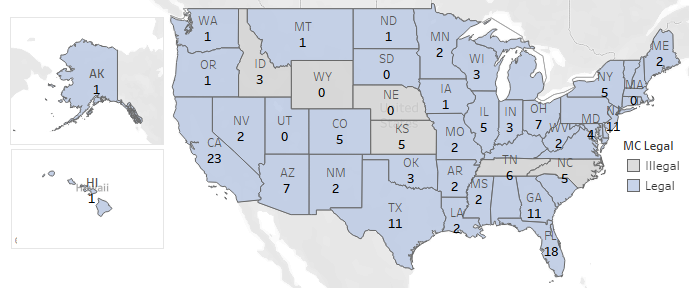
\includegraphics{participants_map.png}

\hypertarget{data-analysis}{%
\section{Data Analysis}\label{data-analysis}}

\hypertarget{attrition-analysis}{%
\subsection{Attrition Analysis}\label{attrition-analysis}}

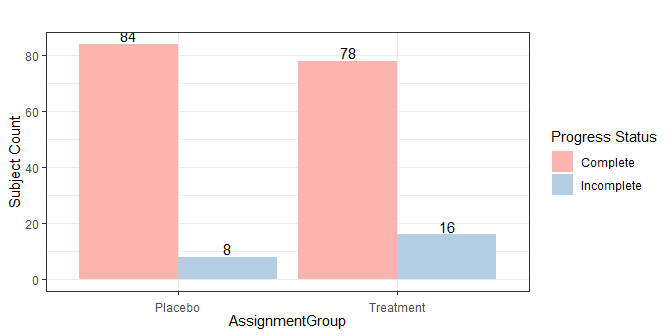
\includegraphics{FullExperiment_files/figure-latex/unnamed-chunk-12-1.pdf}

\begin{verbatim}
           
            Complete Incomplete
  Placebo         84          8
  Treatment       78         16
\end{verbatim}

\begin{verbatim}

    Pearson's Chi-squared test with Yates' continuity correction

data:  assignmentgroup_progress
X-squared = 2.1747, df = 1, p-value = 0.1403
\end{verbatim}

\emph{Missing participant estimates based on covariates using
regression}

\begin{longtable}[]{@{}lrr@{}}
\toprule
& Placebo & Treatment\tabularnewline
\midrule
\endhead
(Intercept) & 0.230 (0.223) & -0.440\textbf{\texttt{*}}
(0.219)\tabularnewline
ChronicPain & 0.063 (0.042) & 0.041 (0.087)\tabularnewline
OpioidsDeathsInc & -0.023 (0.029) & 0.070 (0.046)\tabularnewline
Gender\_Female & 0.094 (0.069) & 0.155\textbf{. } (0.087)\tabularnewline
AgeGroup.L & -0.117\textbf{. } (0.062) & 0.105 (0.074)\tabularnewline
AgeGroup.Q & -0.028 (0.062) & 0.004 (0.078)\tabularnewline
AgeGroup.C & -0.066 (0.062) & -0.046 (0.079)\tabularnewline
Education.L & 0.055\textbf{. } (0.031) & -0.076 (0.107)\tabularnewline
Education.Q & -0.145 (0.091) & 0.036 (0.096)\tabularnewline
Employed\_Yes & -0.180 (0.128) & 0.207\textbf{\texttt{**}}
(0.072)\tabularnewline
PoliticalBelief\_Conservative & 0.069 (0.062) & 0.018
(0.086)\tabularnewline
PoliticalBelief\_Ind./Other & 0.034 (0.075) & 0.140
(0.107)\tabularnewline
Ethnicity\_Black or African Am & 0.218 (0.188) & 0.047
(0.120)\tabularnewline
Ethnicity\_Hispanic/Latino & -0.078 (0.062) & 0.143
(0.128)\tabularnewline
Ethnicity\_Asian & -0.122 (0.091) & -0.155 (0.121)\tabularnewline
Ethnicity\_Other & -0.102 (0.083) & -0.096 (0.115)\tabularnewline
\bottomrule
\end{longtable}

\emph{Extreme Values Bounds}

\begin{verbatim}
           
            No Yes
  Placebo   11  81
  Treatment 11  83
\end{verbatim}

\begin{verbatim}
           
            No Yes
  Placebo    2   6
  Treatment  0  16
\end{verbatim}

Total participants count is \textbf{186}. Total participants who didn't
finish the Survey is \textbf{24}. Participants count after excluding
attrition is \textbf{162}.

\hypertarget{non-u.s.-participants}{%
\subsection{Non-U.S. participants}\label{non-u.s.-participants}}

We will make sure that the participants are from US location by checking
the Qualtrics metadata information.

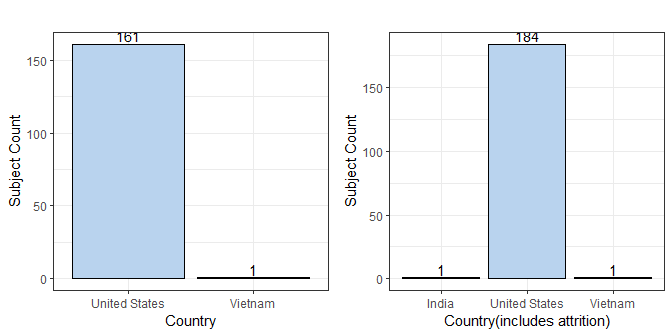
\includegraphics{FullExperiment_files/figure-latex/unnamed-chunk-21-1.pdf}

\hypertarget{bots}{%
\subsection{Bots}\label{bots}}

Include a CAPTCHA at the beginning to prevent bots from taking the
Survey. Qualtrics uses Google reCAPTCHA technology. According to
Qualtrics, if the score is less than 0.5, the response can be flagged as
a bot. We will filter out participants where the CAPTCHA score is less
than 0.5.

Total participants count is \textbf{161}. Total participants with
CAPTCHA score less than 0.5 are \textbf{5}. Participants count after
removal of less CAPTCHA score is \textbf{156}.

Total participants with CAPTCHA score less than 0.5 (includes attrition
data) are \textbf{5}. Participants count after removal of less CAPTCHA
score is \textbf{179}.

\hypertarget{exceptionally-fast-outliers}{%
\subsection{Exceptionally fast
outliers}\label{exceptionally-fast-outliers}}

Based on the Participants' total time taken to complete the Survey,
filter out data from the Participants who are statistical outliers (1
standard deviations below the mean of the time taken). Since our videos
in treatment and placebo groups will have equal time, we will also
compare these outliers between the treatment and placebo groups to check
for any abnormality. Note: Initially, we thought of using attention
check questions, since there is a threat of post-treatment bias, we did
not use those.

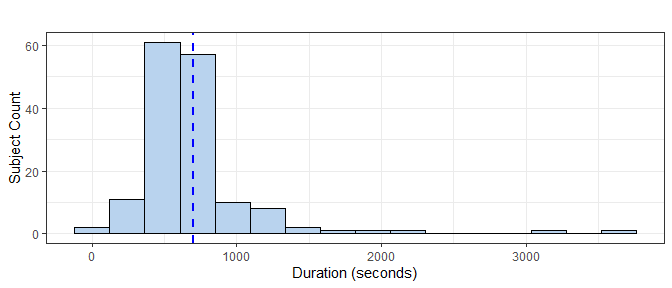
\includegraphics{FullExperiment_files/figure-latex/unnamed-chunk-26-1.pdf}

\begin{longtable}[]{@{}rlll@{}}
\toprule
Duration & AssignmentGroup & AgeGroup & ResponseId\tabularnewline
\midrule
\endhead
201 & Treatment & 25-35 & R\_3MPEFlTXmTxsDPu\tabularnewline
226 & Treatment & 25-35 & R\_2YhLXXgz5B2uCGv\tabularnewline
54 & Placebo & 25-35 & R\_RrX64Mgir5Vs3Dz\tabularnewline
222 & Treatment & 25-35 & R\_pugyP51UV2yJRol\tabularnewline
77 & Placebo & 25-35 & R\_DSv0t38U0NrcFDH\tabularnewline
153 & Treatment & 25-35 & R\_1lsheWGWjxQ2raE\tabularnewline
215 & Placebo & 35-45 & R\_2h1FNXe7uNMA2jf\tabularnewline
210 & Treatment & 45-55 & R\_2QXNDX6JrcyS6cZ\tabularnewline
\bottomrule
\end{longtable}

Exceptionally fast outliers count is \textbf{8}.

Exceptionally fast outliers (includes attrition data) count is
\textbf{8}.

\hypertarget{duplicate-participants}{%
\subsection{Duplicate participants}\label{duplicate-participants}}

We apply due diligence to find out duplicate participants by checking
the hashed IP address and similarity in covariates and filter them out.

\begin{verbatim}
Duplicate IP addresses (Includes attrition data) 
\end{verbatim}

\begin{longtable}[]{@{}lllll@{}}
\toprule
AssignmentGroup & Gender & AgeGroup & Region & ResponseId\tabularnewline
\midrule
\endhead
Placebo & Female & 55 and Older & ID & R\_1CEGVKUl8Gfcp8U\tabularnewline
Placebo & Male & 55 and Older & ID & FS\_ezzaqDq7Q40j6sF\tabularnewline
\bottomrule
\end{longtable}

Total participants after filtering are \textbf{148}.\\
Total participants after filtering (includes attrition data) are
\textbf{169}.

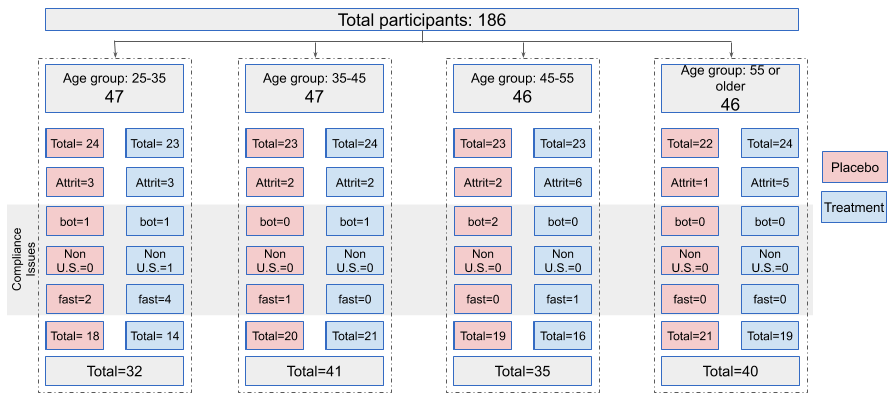
\includegraphics{participants_group.png}

\hypertarget{covariate-balance-check}{%
\subsection{Covariate Balance Check}\label{covariate-balance-check}}

Much of the analysis we do relies on the assumption that (except for
some key characteristics) participants are random. By `random', we mean
that participants have random personal backgrounds and histories
(e.g.~race, religion, political affiliation) and that there is not a
strong presence of one background over another in our subject sample.

Practically, it is impossible to enforce complete randomization.
Consequently, in order for our assumption of complete randomness to hold
true, we now conduct a covariate balance check. The purpose of the
covariate balance check is to ensure that we have relatively balanced
responses to each of the potential covariates that we have identified in
this study. For the purposes of this covraiate balance check, we will
examine the factorized version of the covariates only.

It is important to note that age ranges are automatically balanced
because we blocked with an equal number of participants in each age
group and were able to enforce those blocks thanks to MTurk.

To increase our confidence, we also employ Bartlett's test for
homogeneity of variances. This test will allow us to see if there is
different variation between the variables. The null hypothesis will be
that the variance is equal for all variables, so if we can reject this
null hypothesis then we can be more confident in the fact that the
covariates are balanced.

Please note that we will run these tests on each of the three data
tables that we have due to our handling of the extreme value bounds. One
table removed extreme values, one replaced these values with the lowest
value, and one replaced these values with the highest value.

\begin{verbatim}

    Bartlett test of homogeneity of variances

data:  d$treated and factor(d$AgeGroup)
Bartlett's K-squared = 0.00062919, df = 3, p-value = 1
\end{verbatim}

\begin{verbatim}

    Bartlett test of homogeneity of variances

data:  d$treated and factor(d$ChronicPain)
Bartlett's K-squared = 0.00070285, df = 1, p-value = 0.9788
\end{verbatim}

\begin{verbatim}

    Bartlett test of homogeneity of variances

data:  d$treated and factor(d$Employed)
Bartlett's K-squared = 0.012805, df = 1, p-value = 0.9099
\end{verbatim}

We can see from our Bartlett's test of homogeneity of variances that we
cannot reject the null hypothesis that any of these covariates are
homogeneous. The means that we do not have a violation of the
homogeneity of variance between groups with respect to proceeding with
an ANOVA test on the difference in means for our covariates of interest.
This analysis is identical for all three of our tables generated from
our extreme value bounds handling.

With each of the tables, we first ran a Bartlett's test to test the
homogeneity of variance. Found that no violation of homogeneity of
variance, meaning similar variation across groups. This is good because
it indicates there is no statistically significant bias in one group
over another and indicates that randomness likely has worked.

To gain additional confidence, we proceed with an ANOVA test on the
difference in means for our covariates of interest. This analysis is
identical for all three of our tables generated from our extreme value
bounds handling.

\begin{verbatim}
Analysis of Variance Table

Model 1: treated ~ 1 + ChronicPain + Gender + AgeGroup + Education + Employed + 
    PoliticalBelief + Ethnicity
Model 2: treated ~ 1
  Res.Df    RSS  Df Sum of Sq      F Pr(>F)
1    133 32.929                            
2    147 36.892 -14   -3.9626 1.1432 0.3269
\end{verbatim}

In this test, we are checking whether any of the covariates predict to
which assignment group (placebo/treatment) they have been assigned to.
Since the p-value for our F-test is greater than 0.05, we say that this
result is not statistically significant. Since the p-value is not
statistically significant in this ANOVA F-test, then we can say that
randomization has worked!

One note for the reader: we examined whether it was appropriate to use a
difference-in-difference (DID) check to further validate our examination
of the placebo and treatment groups. These techniques typically require
time series data from a control and a treatment group over time to
examine whether there is a difference between the changes in the two
groups over time. Since this experiment does not use any time series
data, we believe that it is not appropriate to use DID techniques for
this experiment, and thus we have not included this sort of analysis in
this paper.

\hypertarget{assignment-and-demographic-data}{%
\subsection{Assignment and Demographic
data}\label{assignment-and-demographic-data}}

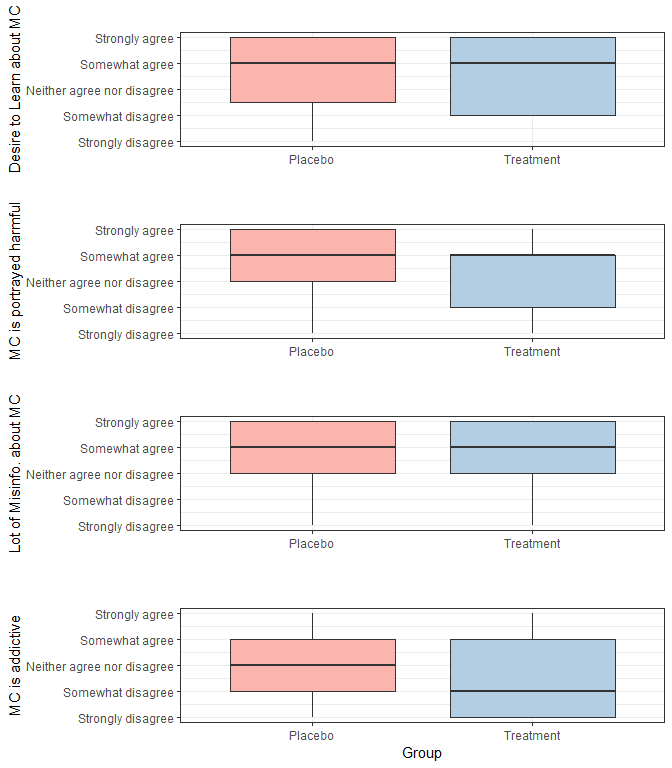
\includegraphics{FullExperiment_files/figure-latex/unnamed-chunk-34-1.pdf}

\hypertarget{eda}{%
\subsection{EDA}\label{eda}}

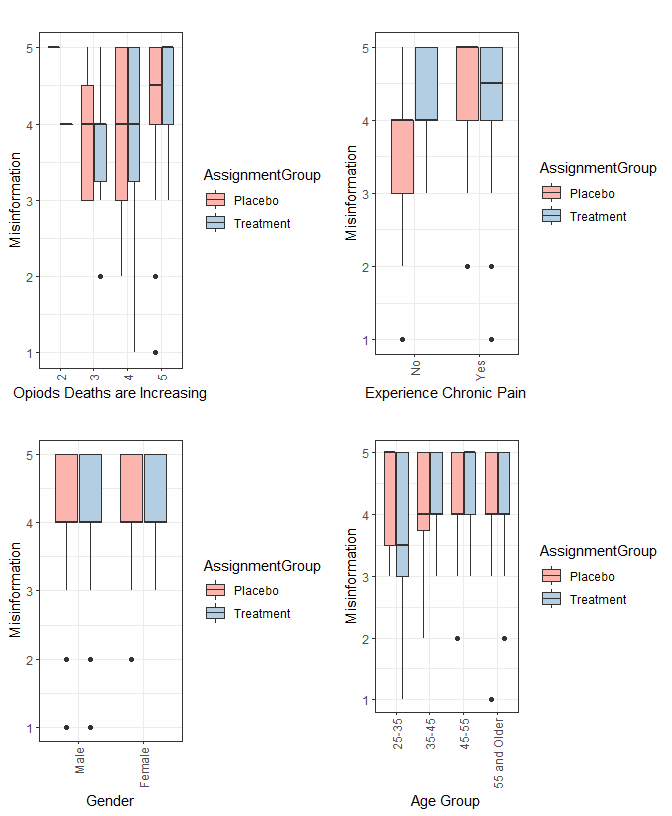
\includegraphics{FullExperiment_files/figure-latex/unnamed-chunk-36-1.pdf}

The major takeaways from these graphs are that none of the variables are
strongly correlated with one another except for two outcome variables:
MC\_MisInfo and MC\_PortrayedHarm. This result is expected - we did not
anticipate `identity variables' such as ethnicity or political
affiliation to strongly affect any of the other variables in this
setting. We also expected the outcome variables to slightly correlate
with one another.

\pagebreak

\textbf{Outcome measures (Excludes Attrition)}

We can now examine our outcome variables in between groups to see how
they vary between control and treatment - we do this for all three
versions of our data table (removing subjects who did not complete
entirely, replacing their data with the lowest value, and replacing
their data with the highest value).

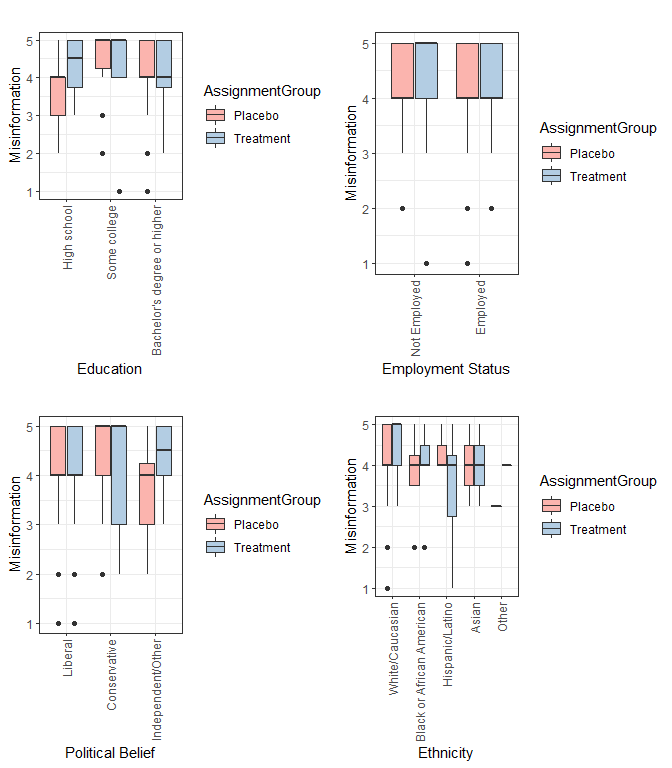
\includegraphics{FullExperiment_files/figure-latex/unnamed-chunk-37-1.pdf}

\pagebreak

\textbf{Outcome measures (Low value bound)}

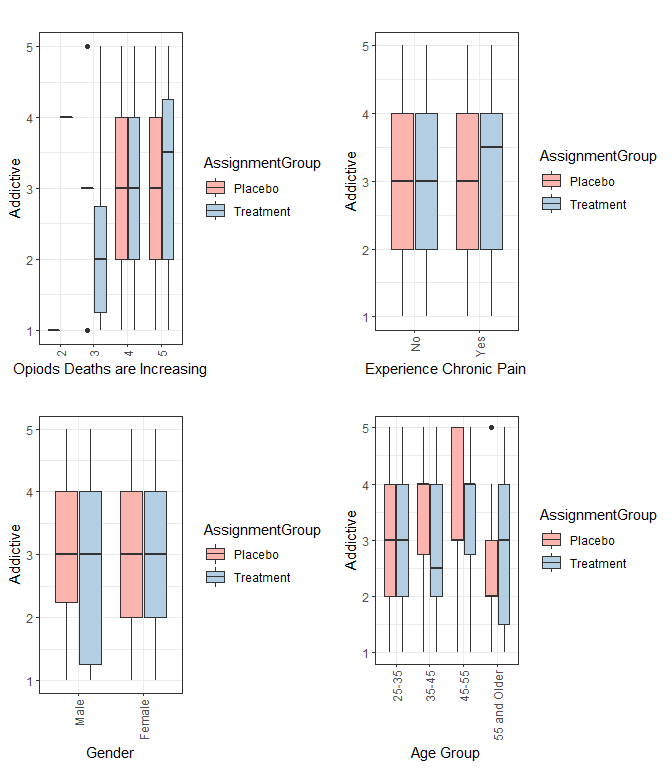
\includegraphics{FullExperiment_files/figure-latex/unnamed-chunk-38-1.pdf}

\pagebreak

\textbf{Outcome measures (High value bound)}

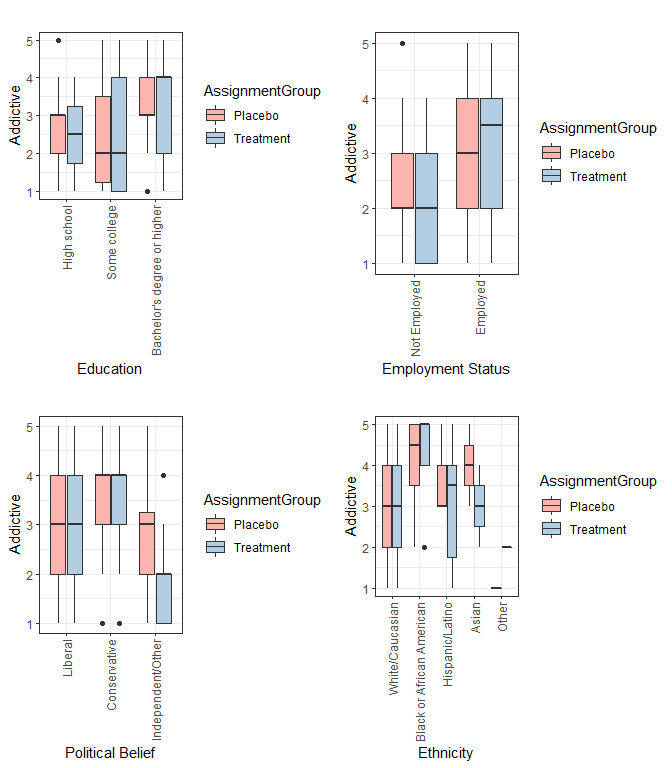
\includegraphics{FullExperiment_files/figure-latex/unnamed-chunk-39-1.pdf}

\pagebreak

Practically, it is impossible to enforce complete randomization.
Consequently, in order for our assumption of complete randomness to hold
true, we now conduct a covariate balance check. The purpose of the
covariate balance check is to ensure that we have relatively balanced
responses to each of the potential covariates that we have identified in
this study. For the purposes of this covariate balance check, we will
examine the factorized version of the covariates only.

\hypertarget{results}{%
\section{Results}\label{results}}

Let us look at the results about the subjects' opinion on our primary
and secondary outcome measures.

\hypertarget{desire-to-learn-about-medical-cannabis}{%
\subsection{Desire to learn about medical
cannabis}\label{desire-to-learn-about-medical-cannabis}}

We are comparing six variants of the model for our primary outcome
measures.

\begin{longtable}[]{@{}ll@{}}
\toprule
\begin{minipage}[b]{0.35\columnwidth}\raggedright
Model\strut
\end{minipage} & \begin{minipage}[b]{0.59\columnwidth}\raggedright
Covariates\strut
\end{minipage}\tabularnewline
\midrule
\endhead
\begin{minipage}[t]{0.35\columnwidth}\raggedright
model\_1\strut
\end{minipage} & \begin{minipage}[t]{0.59\columnwidth}\raggedright
treated\strut
\end{minipage}\tabularnewline
\begin{minipage}[t]{0.35\columnwidth}\raggedright
model\_2\strut
\end{minipage} & \begin{minipage}[t]{0.59\columnwidth}\raggedright
treated + ChronicPain + OpioidsDeathsInc\strut
\end{minipage}\tabularnewline
\begin{minipage}[t]{0.35\columnwidth}\raggedright
model\_3\strut
\end{minipage} & \begin{minipage}[t]{0.59\columnwidth}\raggedright
treated + ChronicPain + OpioidsDeathsInc + ChronicPain*treated\strut
\end{minipage}\tabularnewline
\begin{minipage}[t]{0.35\columnwidth}\raggedright
model\_4\strut
\end{minipage} & \begin{minipage}[t]{0.59\columnwidth}\raggedright
treated + ChronicPain + OpioidsDeathsInc + ChronicPain*treated+
AgeGroup\strut
\end{minipage}\tabularnewline
\begin{minipage}[t]{0.35\columnwidth}\raggedright
model\_5\strut
\end{minipage} & \begin{minipage}[t]{0.59\columnwidth}\raggedright
treated + ChronicPain + OpioidsDeathsInc + ChronicPain*treated+ AgeGroup
+ Gender\strut
\end{minipage}\tabularnewline
\begin{minipage}[t]{0.35\columnwidth}\raggedright
model\_6\strut
\end{minipage} & \begin{minipage}[t]{0.59\columnwidth}\raggedright
treated + ChronicPain + OpioidsDeathsInc + ChronicPain*treated+ AgeGroup
+ Gender +PoliticalBelief\strut
\end{minipage}\tabularnewline
\bottomrule
\end{longtable}

\begin{verbatim}

1) Desire to learn about the benefits of medical cannabis for chronic pain?
----------------------------------------------------------------------------------
                                    Desire to learn about Medical Cannabis        
                              (1)      (2)      (3)       (4)      (5)      (6)   
----------------------------------------------------------------------------------
treated                      0.352*   0.342*   0.625    0.715*    0.692*   0.703* 
                            (0.186)  (0.183)  (0.388)   (0.389)  (0.390)  (0.397) 
ChronicPain                          0.694*** 0.875*** 0.909***  0.918*** 0.915***
                                     (0.222)  (0.326)   (0.320)  (0.320)  (0.324) 
OpioidsDeathsInc                      0.069    0.064     0.078    0.082    0.078  
                                     (0.152)  (0.154)   (0.156)  (0.156)  (0.160) 
treated:ChronicPain                            -0.394   -0.498    -0.476   -0.481 
                                              (0.436)   (0.435)  (0.436)  (0.442) 
AgeGroup.L                                             -0.435*** -0.403** -0.395**
                                                        (0.167)  (0.176)  (0.182) 
AgeGroup.Q                                               0.110    0.106    0.116  
                                                        (0.181)  (0.182)  (0.190) 
AgeGroup.C                                              -0.159    -0.151   -0.148 
                                                        (0.190)  (0.190)  (0.193) 
GenderFemale                                                      -0.154   -0.166 
                                                                 (0.193)  (0.200) 
PoliticalBeliefConservative                                                -0.047 
                                                                          (0.216) 
PoliticalBeliefInd./Other                                                  -0.123 
                                                                          (0.293) 
Constant                    3.833*** 3.038*** 2.932*** 2.858***  2.909*** 2.964***
                            (0.146)  (0.751)  (0.795)   (0.796)  (0.803)  (0.824) 
N                             148      148      148       148      148      148   
R2                           0.024    0.099    0.105     0.144    0.149    0.150  
Adjusted R2                  0.017    0.080    0.080     0.102    0.100    0.088  
F Statistic                  3.531*  5.259*** 4.182*** 3.376***  3.034*** 2.419** 
----------------------------------------------------------------------------------
*p < .1; **p < .05; ***p < .01                                                    
\end{verbatim}

\hypertarget{treatment-effect}{%
\subparagraph{Treatment Effect}\label{treatment-effect}}

We see statistically significant results on the treatment across the all
models (except for model 3).

For all models, we can see that people who were exposed to the
treatment, tend to have more desire to learn about the benefits. This
suggests that our treatment has the intended effect of increased desire
to learn about medical cannabis after presenting scientific information
of its benefits.

\hypertarget{other-observations}{%
\subparagraph{Other Observations}\label{other-observations}}

People who have chronic pain show desire to learn about medical cannabis
(statistically significant results at p \textless{} 0.01). This makes
sense as people who have chronic pain will be more inclined to learn
about possible remedies.

There is a trend we can see where the lower the age the more desire
there is to learn about the benefits (statistically significant results
at p \textless{} 0.01). Younger generations seem to be more curious
about alternative therapies.

\pagebreak

\hypertarget{medical-cannabis-is-portrayed-as-harmful}{%
\subsection{Medical cannabis is portrayed as
harmful}\label{medical-cannabis-is-portrayed-as-harmful}}

We are comparing six variants of the model for the secondary outcome
measures.

\begin{longtable}[]{@{}ll@{}}
\toprule
\begin{minipage}[b]{0.35\columnwidth}\raggedright
Model\strut
\end{minipage} & \begin{minipage}[b]{0.59\columnwidth}\raggedright
Covariates\strut
\end{minipage}\tabularnewline
\midrule
\endhead
\begin{minipage}[t]{0.35\columnwidth}\raggedright
model\_1\strut
\end{minipage} & \begin{minipage}[t]{0.59\columnwidth}\raggedright
treated\strut
\end{minipage}\tabularnewline
\begin{minipage}[t]{0.35\columnwidth}\raggedright
model\_2\strut
\end{minipage} & \begin{minipage}[t]{0.59\columnwidth}\raggedright
treated + ChronicPain + OpioidsDeathsInc\strut
\end{minipage}\tabularnewline
\begin{minipage}[t]{0.35\columnwidth}\raggedright
model\_3\strut
\end{minipage} & \begin{minipage}[t]{0.59\columnwidth}\raggedright
treated + ChronicPain + OpioidsDeathsInc + AgeGroup\strut
\end{minipage}\tabularnewline
\begin{minipage}[t]{0.35\columnwidth}\raggedright
model\_4\strut
\end{minipage} & \begin{minipage}[t]{0.59\columnwidth}\raggedright
treated + ChronicPain + OpioidsDeathsInc + AgeGroup + Gender\strut
\end{minipage}\tabularnewline
\begin{minipage}[t]{0.35\columnwidth}\raggedright
model\_5\strut
\end{minipage} & \begin{minipage}[t]{0.59\columnwidth}\raggedright
treated + ChronicPain + OpioidsDeathsInc + AgeGroup + Gender +
PoliticalBelief\strut
\end{minipage}\tabularnewline
\begin{minipage}[t]{0.35\columnwidth}\raggedright
model\_6\strut
\end{minipage} & \begin{minipage}[t]{0.59\columnwidth}\raggedright
treated + ChronicPain + OpioidsDeathsInc + AgeGroup + Gender +
PoliticalBelief + Ethnicity\strut
\end{minipage}\tabularnewline
\bottomrule
\end{longtable}

\begin{verbatim}

2) Medical cannabis is generally portrayed as more harmful than it actually is
-----------------------------------------------------------------------------------
                                      Medical cannabis portrayed as harmful        
                                (1)      (2)      (3)      (4)      (5)      (6)   
-----------------------------------------------------------------------------------
treated                        -0.095   -0.099   -0.104   -0.113   -0.095   -0.108 
                              (0.188)  (0.189)  (0.191)  (0.192)  (0.195)  (0.208) 
ChronicPain                             0.355    0.383*   0.405*   0.372    0.436* 
                                       (0.224)  (0.229)  (0.233)  (0.257)  (0.263) 
OpioidsDeathsInc                        0.043    0.058    0.062    0.058    0.032  
                                       (0.167)  (0.166)  (0.164)  (0.162)  (0.175) 
AgeGroup.L                                       -0.218   -0.183   -0.158   -0.162 
                                                (0.187)  (0.188)  (0.194)  (0.194) 
AgeGroup.Q                                       0.083    0.081    0.108    0.146  
                                                (0.193)  (0.194)  (0.203)  (0.214) 
AgeGroup.C                                       0.207    0.216    0.221    0.204  
                                                (0.202)  (0.201)  (0.202)  (0.215) 
GenderFemale                                              -0.175   -0.209   -0.167 
                                                         (0.195)  (0.197)  (0.199) 
PoliticalBeliefConservative                                        -0.061   -0.076 
                                                                  (0.208)  (0.221) 
PoliticalBeliefInd./Other                                          -0.325   -0.308 
                                                                  (0.308)  (0.307) 
EthnicityBlack or African Am.                                              0.636** 
                                                                           (0.259) 
EthnicityHispanic/Latino                                                    -0.123 
                                                                           (0.418) 
EthnicityAsian                                                              0.079  
                                                                           (0.811) 
EthnicityOther                                                              -0.200 
                                                                           (2.372) 
Constant                      3.795*** 3.352*** 3.267*** 3.318*** 3.439*** 3.467***
                              (0.125)  (0.782)  (0.781)  (0.764)  (0.782)  (0.826) 
N                               148      148      148      148      148      148   
R2                             0.002    0.022    0.041    0.046    0.056    0.076  
Adjusted R2                    -0.005   0.002   -0.0001   -0.001   -0.006   -0.013 
F Statistic                    0.259    1.095    0.997    0.973    0.906    0.851  
-----------------------------------------------------------------------------------
*p < .1; **p < .05; ***p < .01                                                     
\end{verbatim}

\hypertarget{treatment-effect-1}{%
\subparagraph{Treatment Effect}\label{treatment-effect-1}}

People who were exposed to the treatment tend to \emph{disagree} more
that medical cannabis is generally portrayed as harmful than it actually
is.

\hypertarget{other-observations-1}{%
\subparagraph{Other Observations}\label{other-observations-1}}

People who have chronic pain strongly \emph{agree} more than others.
This could be because people who have experienced chronic pain are more
motivated to try out medical cannabis.

We see heterogeneous effects in different ethnic sub-groups. African
Americans strongly \emph{agree} more than others (statistically
significant results at p \textless{} 0.05 - model 6).

\pagebreak

\hypertarget{there-is-a-lot-of-misinformation}{%
\subsection{There is a lot of
misinformation}\label{there-is-a-lot-of-misinformation}}

We are comparing six variants of the model as mentioned above for the
secondary outcome measure.

\begin{verbatim}

3) There is a lot of misinformation about medical cannabis
-----------------------------------------------------------------------------------
                                      Misinformation about medical cannabis        
                                (1)      (2)      (3)      (4)      (5)      (6)   
-----------------------------------------------------------------------------------
treated                        0.142    0.153    0.146    0.146    0.141    0.206  
                              (0.149)  (0.147)  (0.153)  (0.154)  (0.157)  (0.156) 
ChronicPain                             0.299*   0.314*   0.314*   0.298*  0.352** 
                                       (0.167)  (0.167)  (0.171)  (0.176)  (0.177) 
OpioidsDeathsInc                        0.199*   0.208*   0.208*   0.213*   0.206* 
                                       (0.110)  (0.110)  (0.111)  (0.113)  (0.114) 
AgeGroup.L                                       0.006    0.006    0.006    -0.015 
                                                (0.166)  (0.171)  (0.177)  (0.172) 
AgeGroup.Q                                       -0.140   -0.140   -0.141   -0.204 
                                                (0.156)  (0.156)  (0.165)  (0.168) 
AgeGroup.C                                       0.057    0.057    0.055    0.034  
                                                (0.142)  (0.145)  (0.146)  (0.152) 
GenderFemale                                              0.001    0.001    -0.030 
                                                         (0.158)  (0.169)  (0.182) 
PoliticalBeliefConservative                                        0.066    0.068  
                                                                  (0.173)  (0.173) 
PoliticalBeliefInd./Other                                          0.036    -0.018 
                                                                  (0.242)  (0.247) 
EthnicityBlack or African Am.                                               -0.231 
                                                                           (0.313) 
EthnicityHispanic/Latino                                                   -0.708* 
                                                                           (0.415) 
EthnicityAsian                                                              -0.210 
                                                                           (0.458) 
EthnicityOther                                                              -0.884 
                                                                           (0.842) 
Constant                      4.115*** 3.018*** 2.965*** 2.965*** 2.927*** 3.000***
                              (0.107)  (0.524)  (0.518)  (0.529)  (0.560)  (0.565) 
N                               148      148      148      148      148      148   
R2                             0.006    0.049    0.056    0.056    0.057    0.108  
Adjusted R2                    -0.001   0.029    0.016    0.009    -0.004   0.022  
F Statistic                    0.907    2.487*   1.403    1.194    0.933    1.252  
-----------------------------------------------------------------------------------
*p < .1; **p < .05; ***p < .01                                                     
\end{verbatim}

\hypertarget{treatment-effect-2}{%
\subparagraph{Treatment Effect}\label{treatment-effect-2}}

People who were exposed to the treatment tend to \emph{agree} more that
there is a lot of misinformation about medical cannibis.

\hypertarget{other-observations-2}{%
\subparagraph{Other Observations}\label{other-observations-2}}

People who have chronic pain strongly \emph{agree} more than others.
This could be because people who have experienced chronic pain are more
motivated to try out medical cannabis.

People who believe that opiod deaths are increasing more strongly
\emph{agree} that there is a lot of misinformation about medical
cannabis.

Among different ethnic groups, Hispanic/Latino strongly \emph{disagree}
more than other groups.

\pagebreak

\hypertarget{medical-cannabis-is-addictive}{%
\subsection{Medical cannabis is
addictive}\label{medical-cannabis-is-addictive}}

We are comparing six variants of the model as mentioned above for the
secondary outcome measure.

\begin{verbatim}

4) Medical cannabis is addictive
---------------------------------------------------------------------------------
                                         Medical cannabis is addictive           
                                (1)      (2)     (3)      (4)      (5)     (6)   
---------------------------------------------------------------------------------
treated                        -0.051  -0.044   -0.046   -0.048  -0.061   -0.120 
                              (0.224)  (0.224) (0.225)  (0.224)  (0.220) (0.222) 
ChronicPain                            0.454*   0.462*   0.468*   0.198   0.362  
                                       (0.246) (0.241)  (0.243)  (0.271) (0.254) 
OpioidsDeathsInc                        0.204   0.233    0.234    0.282   0.205  
                                       (0.172) (0.170)  (0.171)  (0.172) (0.169) 
AgeGroup.L                                      -0.134   -0.124  -0.059   -0.055 
                                               (0.218)  (0.227)  (0.214) (0.210) 
AgeGroup.Q                                     -0.467** -0.468** -0.409*  -0.345 
                                               (0.221)  (0.223)  (0.225) (0.219) 
AgeGroup.C                                      -0.162   -0.160  -0.170   -0.209 
                                               (0.225)  (0.227)  (0.229) (0.224) 
GenderFemale                                             -0.050  -0.134   -0.011 
                                                        (0.230)  (0.233) (0.236) 
PoliticalBeliefConservative                                      0.602** 0.587** 
                                                                 (0.260) (0.260) 
PoliticalBeliefInd./Other                                        -0.419   -0.399 
                                                                 (0.326) (0.282) 
EthnicityBlack or African Am.                                            1.394** 
                                                                         (0.547) 
EthnicityHispanic/Latino                                                  -0.043 
                                                                         (0.478) 
EthnicityAsian                                                            0.858  
                                                                         (0.578) 
EthnicityOther                                                           -1.760* 
                                                                         (0.940) 
Constant                      3.051*** 1.822** 1.693**  1.707**  1.582*  1.681** 
                              (0.144)  (0.805) (0.801)  (0.811)  (0.845) (0.797) 
N                               148      148     148      148      148     148   
R2                             0.0004   0.033   0.071    0.071    0.137   0.234  
Adjusted R2                    -0.006   0.013   0.031    0.024    0.080   0.160  
F Statistic                    0.054    1.649   1.785    1.527   2.427** 3.153***
---------------------------------------------------------------------------------
*p < .1; **p < .05; ***p < .01                                                   
\end{verbatim}

\hypertarget{treatment-effect-3}{%
\subparagraph{Treatment Effect}\label{treatment-effect-3}}

People who were exposed to the treatment tend to \emph{disagree} more
that medical cannabis is addictive.

\hypertarget{other-observations-3}{%
\subparagraph{Other Observations}\label{other-observations-3}}

People who have chronic pain strongly \emph{agree} more than others.

Younger age groups \emph{disagree} more than others that medical
cannabis is addictive.

Among political affiliations, Conservatives more strongly agree that
medical cannabis is addictive (statistically significant results at p
\textless{} 0.05).

We can see the same trend for African-American ethnic groups.

People who have not reported their ethnicity tend to disagree.

\hypertarget{summary}{%
\subparagraph{Summary}\label{summary}}

People who were exposed to the treatment,

\begin{enumerate}
\def\labelenumi{\arabic{enumi}.}
\item
  show increased desire to learn more about medical cannabis.
\item
  tend to \emph{agree} more that there is a lot of misinformation about
  medical cannibis.
\item
  tend to \emph{disagree} more that medical cannabis is generally
  portrayed as harmful than it actually is.
\item
  tend to \emph{disagree} more that medical cannabis is addictive.
\end{enumerate}

To summarize, our treatment shows a positive effect. Generally, people
do not believe that medical cannabis is addictive, think there is a lot
of misinformation about medical cannabis but do not think it is potrayed
\emph{more} harmful than it actually is.

\hypertarget{posterior-beliefs}{%
\section{Posterior Beliefs}\label{posterior-beliefs}}

Our experimental results show the following about our prior beliefs:\\
1. US residents are interested in learning more about the medical
benefits of cannabis if they know its benefits as the opioids deaths are
increasing.

We did see the intended treatment effect that US residents are
interested in learning more about the medical benefits of cannabis if
they know its benefits. The effect is strongly seen among the younger
adults and people who have experienced chronic pain.

\begin{enumerate}
\def\labelenumi{\arabic{enumi}.}
\setcounter{enumi}{1}
\tightlist
\item
  Cannabis is portrayed as more harmful than it actually is.
\end{enumerate}

We did not see any statistically significant results.

\begin{enumerate}
\def\labelenumi{\arabic{enumi}.}
\setcounter{enumi}{2}
\tightlist
\item
  There is a lot of misinformation about medical cannabis.
\end{enumerate}

We did not see any statistically significant results.

\begin{enumerate}
\def\labelenumi{\arabic{enumi}.}
\setcounter{enumi}{3}
\tightlist
\item
  US residents believe that Medical cannabis is addictive.
\end{enumerate}

We did not see any statistically significant results.

However, we see statistically significant results for some sub-groups on
the last three hypothesis that warrants further research.

\hypertarget{limitations}{%
\section{Limitations}\label{limitations}}

Our current experiment has some limitations.

\hypertarget{current-design}{%
\subparagraph{Current design}\label{current-design}}

We are limiting our subjects to users who participate in MTurk. The
subjects pool may not have sufficient variability to represent the
population. For instance, only people who have access to web and who are
interested in side-gig would have taken the survey.

Also, the youngest age-group 21-24 are not part of this community and
won't be able to participate in the survey. This implies that our
experimental results may not be valid for American adults aged 21-24

\hypertarget{omitted-variables}{%
\subparagraph{Omitted Variables}\label{omitted-variables}}

There could be many important covariates that we have not measured that
could help us in gain precision in our treatment effect estimates.

For example: the kind of chronic pain, its duration and intensity would
influence the outcome measures.

Any first hand experience with chronic pain, substance abuse or
painkillers either by self or within the family or friends could
strongly influence the outcome measures.

These could increase our statistical power when included. Some of these
could be unobservables due to privacy, ethical or legal concerns.

\hypertarget{convenience-sampling}{%
\subparagraph{Convenience Sampling}\label{convenience-sampling}}

There could also be bias due to convenience sampling in our study as we
are using MTurk only. Even for statistically significant results, we
cannot know for sure why our treatment worked.

We need to do sub-group analysis and ``Implicit mediation'' analysis for
further understanding the causal relationships.

\hypertarget{spillovers}{%
\section{Spillovers}\label{spillovers}}

The Spillover effect for our experiment should be inconsequential due to
our experimental design.

The survey was done within a timespan of few hours over a weekend. We
also did ip-based filtering to allow only one entry per IP address.

These measures should ensure spillover effects are under control.

\hypertarget{generalizability}{%
\section{Generalizability}\label{generalizability}}

Our experiment setup should be generalizable for similar social science
research questions.

The setup satisfies the constraints of experimental design which are :
Random Sampling, Excludability and Non-Interference

However, the results may not be generalizable and would require further
studies to understand heterogeneity among different sub-groups and their
treatment effects.

\hypertarget{future-steps}{%
\section{Future Steps}\label{future-steps}}

As a follow up, additional details on the chronic pain such as severity
and duration will further enrich the model and provide important
insights.

The experiment should include questionnaires that captures information
to deduce socio economic status, family size and household income.

We also believe that including subjects with age group: 21-24 is
important to study the effects on the younger adults.

\hypertarget{conclusion}{%
\section{Conclusion}\label{conclusion}}

We started with four hypothesis regarding the perception about medical
cannabis.

Our experiment was able to find statistically significant result that
supports one of our hypothesis that subjects showed positive interest in
learning about medical marujiana after showing them scientific
information about its benefits.

As expected, applying the treatment on a subject generally causes that
subject to view medical cannabis more favorably. The participants in the
treatment group agree more about the benefits of medical cannabis on
chronic pain and believe that there is lot of misinformation about
medical cannabis. They also tend to agree more that medical cannabis is
NOT addictive.

One element to consider in this analysis is the potential for omitted
variable bias. Omitted variable bias occurs when the researchers do not
control for a covariate that might correlate with the treatment effect.
In this case, the researchers controlled for several elements (e.g.~age)
that we felt might cause a correlation with the treatment effect. Having
said that, we recognized that there are several potential variables that
we did not examine that could have an effect on the measured treatment
effect. For example there are several `chronic pain variables' that we
did not explicitly measure, such as duration of pain, intensity of pain,
and type of pain. We also chose not to measure a subject's history with
painkillers, as we were concerned about the potential ethics of asking
for and storing this personal medical information. These variables would
be if a subject is already a medical cannabis user, if the subject is
already on an opiate, if the subject is already using a third type of
painkiller. Although these variables could potentially lead to some sort
of omitted variable bias, we are confident that such bias is likely
relatively low since we controlled for the most important variables
already.

We had to deal with other general issues such as attrition. We were able
to handle attrition using extreme value bounds.

The platform we used for our experimental study was MTurk for several
reasons such as convenience, speed and availability. But we want to also
acknowledge the limitation of this platform and the bias that is leads
to.

A good future extension of our work should look into optimal ways to
extend and generalize while minimizing bias.

\hypertarget{references}{%
\section{References}\label{references}}

{[}1{]} September is Pain Awareness Month. (n.d.). The ACPA.
\url{https://www.theacpa.org/pain-awareness/september-is-pain-awareness-month/}\\
{[}2{]} Dahlhamer, J., Lucas, J., Zelaya, C., \& Nahin, R. (2018). CDC:
Prevalence of Chronic Pain Among U.S. Adults. MMWR. Morbidity and
Mortality Weekly Report, 67(36), 1001--1006.
\url{https://doi.org/10.15585/mmwr.mm6736a2}\\
{[}3{]} U.S. Department of Health and Human Services. (2014).
Healthypeople.Gov. \url{https://www.healthypeople.gov/}\\
{[}4{]} Rosenblum, A., Marsch, L. A., Joseph, H., \& Portenoy, R. K.
(2008). NIH: Opioids and the Treatment of Chronic Pain. Experimental and
Clinical Psychopharmacology, 16(5), 405--416.
\url{https://doi.org/10.1037/a0013628}\\
{[}5{]} CDC: Opioid Overdose in U.S. (2019).
\url{https://www.cdc.gov/drugoverdose/data/prescribing/overview.html}\\
{[}6{]} NIH: Cannabis (Marijuana) - What You Need To Know. (2018,
October 25). NCCIH; NCCIH.
\url{https://nccih.nih.gov/health/marijuana}\\
{[}7{]} Virginia, Y. C. T., BS Pharm, RPh Clinical Pharmacist/Freelance
Medical Writer Haymarket. (n.d.). Medical Cannabis for Chronic Pain.
Www.Uspharmacist.com.
\url{https://www.uspharmacist.com/article/medical-cannabis-for-chronic-pain}\\
{[}8{]} WHO: Global Cannabis consumption. (n.d.). www.Who.Int. Retrieved
December 12, 2020, from
\url{http://www.who.int/substance_abuse/facts/cannabis/en}\\
{[}9{]} Map of Marijuana Legality by State. (2019, February 18).
Marijuana Legality; DISA.
\url{https://disa.com/map-of-marijuana-legality-by-state}\\
{[}10{]} Amazon Mechanical Turk. (2018). Mturk.com.
\url{https://www.mturk.com/}\\
{[}11{]} Cannabis laws by state. (2016). Weedmaps.
\url{https://weedmaps.com/learn/laws-and-regulations/}\\
{[}12{]} HHS: Poverty guidelines and poverty. (2015, November 23). HHS.
\url{https://aspe.hhs.gov/frequently-asked-questions-related-poverty-guidelines-and-poverty}\\
{[}13{]} M.K, W. (2020, March 10). The Research Methods Knowledge Base.
Conjointly.com; Conjoint.ly.
\url{https://conjointly.com/kb/types-of-survey-questions/}\\
{[}14{]} CDC: Chronic Pain Among U.S. Adults, 2019. (2020, November 4).
CDC.gov. \url{https://www.cdc.gov/nchs/products/databriefs/db390.htm}\\
{[}15{]} Lovett, M., Bajaba, S., Lovett, M., \& Simmering, M. J. (2017).
Data Quality from Crowdsourced Surveys. Applied Psychology, 67(2),
339--366. \url{https://doi.org/10.1111/apps.12124}

\hypertarget{appendix}{%
\section{Appendix}\label{appendix}}

\hypertarget{questions}{%
\subsection{Questions}\label{questions}}

\textbf{1. What is your Gender?}

\begin{itemize}
\tightlist
\item
  Male
\item
  Female
\item
  Other
\end{itemize}

\textbf{2. Please specify your ethnicity}

\begin{itemize}
\tightlist
\item
  White
\item
  Black or African American
\item
  Hispanic/Latino
\item
  Asian
\item
  Other
\end{itemize}

\textbf{3. What is the highest level of school you have completed or the
highest degree you have received?}

\begin{itemize}
\tightlist
\item
  Less than high school
\item
  High school
\item
  Some college
\item
  Bachelor's degree or higher
\end{itemize}

\textbf{4. What is your Employment status?}

\begin{itemize}
\tightlist
\item
  Employed
\item
  Not Employed
\end{itemize}

\textbf{5. In general, how would you classify your political beliefs?}

\begin{itemize}
\tightlist
\item
  Liberal
\item
  Conservative
\item
  Independent/Other
\end{itemize}

\textbf{6. Do you experience chronic pain?}

\begin{itemize}
\tightlist
\item
  Yes
\item
  No
\end{itemize}

\hypertarget{baseline-question}{%
\subsubsection{Baseline question}\label{baseline-question}}

\textbf{7. Deaths due to overdoses involving prescription opioids are
increasing.}

\begin{itemize}
\tightlist
\item
  Strongly agree
\item
  Somewhat agree
\item
  Neither agree nor disagree
\item
  Somewhat disagree
\item
  Strongly disagree
\end{itemize}

\hypertarget{outcome-questions}{%
\subsubsection{Outcome questions}\label{outcome-questions}}

\textbf{8. Do you have a desire to learn about the benefits of medical
cannabis for chronic pain?}

\begin{itemize}
\tightlist
\item
  Strongly agree
\item
  Somewhat agree
\item
  Neither agree nor disagree
\item
  Somewhat disagree
\item
  Strongly disagree
\end{itemize}

\textbf{9. Medical cannabis is generally portrayed as more harmful than
it actually is}

\begin{itemize}
\tightlist
\item
  Strongly agree
\item
  Somewhat agree
\item
  Neither agree nor disagree
\item
  Somewhat disagree
\item
  Strongly disagree
\end{itemize}

\textbf{10. There is a lot of misinformation about medical cannabis}

\begin{itemize}
\tightlist
\item
  Strongly agree
\item
  Somewhat agree
\item
  Neither agree nor disagree
\item
  Somewhat disagree
\item
  Strongly disagree
\end{itemize}

\textbf{11. Medical cannabis is addictive}

\begin{itemize}
\tightlist
\item
  Strongly agree
\item
  Somewhat agree
\item
  Neither agree nor disagree
\item
  Somewhat disagree
\item
  Strongly disagree
\end{itemize}

\hypertarget{videos}{%
\subsection{Videos}\label{videos}}

\hypertarget{both-treatment-and-placebo-groups-opioids---risks-and-side-effects}{%
\subsubsection{Both Treatment and Placebo groups (Opioids - Risks and
Side
effects)}\label{both-treatment-and-placebo-groups-opioids---risks-and-side-effects}}

\href{https://youtu.be/y0mfzDAs1BE}{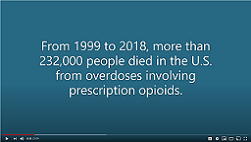
\includegraphics{opioids.png}}

\hypertarget{treatment-group-benefits-of-medical-cannabis}{%
\subsubsection{Treatment group (Benefits of Medical
Cannabis)}\label{treatment-group-benefits-of-medical-cannabis}}

\href{https://youtu.be/OhJ0YaJXrJo}{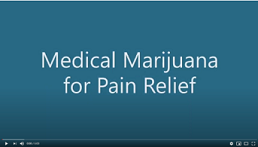
\includegraphics{medical_marijuana.png}}

\hypertarget{placebo-group-benefits-of-cycling}{%
\subsubsection{Placebo group (Benefits of
Cycling)}\label{placebo-group-benefits-of-cycling}}

\href{https://youtu.be/xWo0FOwZVX0}{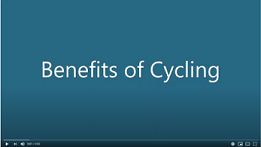
\includegraphics{cycling.png}}

\pagebreak

\hypertarget{models-with-extreme-value-bounds}{%
\subsection{Models with Extreme Value
Bounds}\label{models-with-extreme-value-bounds}}

\begin{verbatim}

1) Desire to learn about the benefits of medical cannabis for chronic pain?
--------------------------------------------------------------------------------------
                                  Desire to learn about Medical Cannabis              
                    Non-attriters | Non-attriters | Low value bound | High value bound
                         (1)             (2)              (3)              (4)        
--------------------------------------------------------------------------------------
treated                0.352*          0.692*            0.415           0.857***     
                       (0.186)         (0.390)          (0.386)          (0.320)      
treated:ChronicPain                    -0.476           -0.382            -0.549      
                                       (0.436)          (0.453)          (0.374)      
ChronicPain                           0.918***          0.660**          0.954***     
                                       (0.320)          (0.327)          (0.260)      
OpioidsDeathsInc                        0.082            0.007            0.089       
                                       (0.156)          (0.157)          (0.122)      
AgeGroup.L                            -0.403**          -0.301           -0.387**     
                                       (0.176)          (0.203)          (0.168)      
AgeGroup.Q                              0.106            0.089            0.081       
                                       (0.182)          (0.204)          (0.166)      
AgeGroup.C                             -0.151            0.051            -0.222      
                                       (0.190)          (0.208)          (0.161)      
GenderFemale                           -0.154           -0.378*           -0.069      
                                       (0.193)          (0.211)          (0.166)      
Constant              3.833***        2.909***         3.328***          2.849***     
                       (0.146)         (0.803)          (0.796)          (0.592)      
N                        148             148              169              169        
R2                      0.024           0.149            0.068            0.168       
Adjusted R2             0.017           0.100            0.022            0.126       
F Statistic            3.531*         3.034***           1.469           4.027***     
--------------------------------------------------------------------------------------
*p < .1; **p < .05; ***p < .01                                                        
\end{verbatim}

TODO: Analysis

\pagebreak

\begin{verbatim}

2) Medical cannabis is generally portrayed as more harmful than it actually is
------------------------------------------------------------------------------------------------
                                            Medical cannabis portrayed as harmful               
                              Non-attriters | Non-attriters | Low value bound | High value bound
                                   (1)             (2)              (3)              (4)        
------------------------------------------------------------------------------------------------
treated                          -0.095          -0.108           -0.334            0.073       
                                 (0.188)         (0.208)          (0.233)          (0.181)      
ChronicPain                                      0.436*            0.220           0.463**      
                                                 (0.263)          (0.286)          (0.218)      
OpioidsDeathsInc                                  0.032           -0.064            0.057       
                                                 (0.175)          (0.170)          (0.136)      
GenderFemale                                     -0.167           -0.450*           0.008       
                                                 (0.199)          (0.231)          (0.186)      
AgeGroup.L                                       -0.162           -0.112            -0.159      
                                                 (0.194)          (0.229)          (0.183)      
AgeGroup.Q                                        0.146            0.104            0.097       
                                                 (0.214)          (0.233)          (0.182)      
AgeGroup.C                                        0.204           0.382*            0.065       
                                                 (0.215)          (0.228)          (0.177)      
PoliticalBeliefConservative                      -0.076           -0.149            -0.054      
                                                 (0.221)          (0.250)          (0.203)      
PoliticalBeliefInd./Other                        -0.308           -0.432            -0.177      
                                                 (0.307)          (0.324)          (0.268)      
EthnicityBlack or African Am.                    0.636**           0.064            0.655*      
                                                 (0.259)          (0.489)          (0.349)      
EthnicityHispanic/Latino                         -0.123           -0.228            -0.009      
                                                 (0.418)          (0.422)          (0.341)      
EthnicityAsian                                    0.079            0.350            -0.122      
                                                 (0.811)          (0.917)          (0.532)      
EthnicityOther                                   -0.200            0.226            -0.450      
                                                 (2.372)          (2.440)          (0.829)      
Constant                        3.795***        3.467***         4.053***          3.291***     
                                 (0.125)         (0.826)          (0.808)          (0.652)      
N                                  148             148              169              169        
R2                                0.002           0.076            0.082            0.067       
Adjusted R2                      -0.005          -0.013            0.005            -0.011      
F Statistic                       0.259           0.851            1.071            0.861       
------------------------------------------------------------------------------------------------
*p < .1; **p < .05; ***p < .01                                                                  
\end{verbatim}

TODO: Analysis

\pagebreak

\begin{verbatim}

3) There is a lot of misinformation about medical cannabis
------------------------------------------------------------------------------------------------
                                            Misinformation about medical cannabis               
                              Non-attriters | Non-attriters | Low value bound | High value bound
                                   (1)             (2)              (3)              (4)        
------------------------------------------------------------------------------------------------
treated                           0.142           0.206           -0.032           0.282**      
                                 (0.149)         (0.156)          (0.176)          (0.137)      
OpioidsDeathsInc                                 0.206*            0.168           0.214**      
                                                 (0.114)          (0.119)          (0.103)      
ChronicPain                                      0.352**           0.147           0.368**      
                                                 (0.177)          (0.203)          (0.165)      
GenderFemale                                     -0.030           -0.261            0.079       
                                                 (0.182)          (0.191)          (0.141)      
AgeGroup.L                                       -0.015            0.064            -0.046      
                                                 (0.172)          (0.200)          (0.139)      
AgeGroup.Q                                       -0.204           -0.286            -0.205      
                                                 (0.168)          (0.182)          (0.138)      
AgeGroup.C                                        0.034            0.133            -0.056      
                                                 (0.152)          (0.161)          (0.134)      
PoliticalBeliefConservative                       0.068           -0.009            0.081       
                                                 (0.173)          (0.188)          (0.154)      
PoliticalBeliefInd./Other                        -0.018           -0.308            0.012       
                                                 (0.247)          (0.299)          (0.203)      
EthnicityBlack or African Am.                    -0.231           -0.317            -0.076      
                                                 (0.313)          (0.276)          (0.264)      
EthnicityHispanic/Latino                         -0.708*          -0.549           -0.571**     
                                                 (0.415)          (0.348)          (0.259)      
EthnicityAsian                                   -0.210            0.072            -0.291      
                                                 (0.458)          (0.545)          (0.403)      
EthnicityOther                                   -0.884           -0.532            -1.010      
                                                 (0.842)          (0.946)          (0.628)      
Constant                        4.115***        3.000***         3.352***          2.924***     
                                 (0.107)         (0.565)          (0.578)          (0.494)      
N                                  148             148              169              169        
R2                                0.006           0.108            0.067            0.119       
Adjusted R2                      -0.001           0.022           -0.011            0.045       
F Statistic                       0.907           1.252            0.856            1.611*      
------------------------------------------------------------------------------------------------
*p < .1; **p < .05; ***p < .01                                                                  
\end{verbatim}

TODO: Analysis

\pagebreak

\begin{verbatim}

4) Medical cannabis is addictive
------------------------------------------------------------------------------------------------
                                                Medical cannabis is addictive                   
                              Non-attriters | Non-attriters | Low value bound | High value bound
                                   (1)             (2)              (3)              (4)        
------------------------------------------------------------------------------------------------
treated                          -0.051          -0.120           -0.283            0.152       
                                 (0.224)         (0.222)          (0.233)          (0.207)      
OpioidsDeathsInc                                  0.205            0.120            0.232       
                                                 (0.169)          (0.178)          (0.155)      
ChronicPain                                       0.362            0.217           0.501**      
                                                 (0.254)          (0.254)          (0.249)      
GenderFemale                                     -0.011           -0.266            0.235       
                                                 (0.236)          (0.247)          (0.213)      
AgeGroup.L                                       -0.055            0.006            -0.109      
                                                 (0.210)          (0.224)          (0.209)      
AgeGroup.Q                                       -0.345           -0.385*          -0.373*      
                                                 (0.219)          (0.228)          (0.208)      
AgeGroup.C                                       -0.209            0.009            -0.310      
                                                 (0.224)          (0.231)          (0.203)      
PoliticalBeliefConservative                      0.587**           0.431           0.514**      
                                                 (0.260)          (0.269)          (0.232)      
PoliticalBeliefInd./Other                        -0.399           -0.528*           -0.202      
                                                 (0.282)          (0.301)          (0.306)      
EthnicityBlack or African Am.                    1.394**           0.675           1.259***     
                                                 (0.547)          (0.618)          (0.399)      
EthnicityHispanic/Latino                         -0.043           -0.164            0.022       
                                                 (0.478)          (0.469)          (0.390)      
EthnicityAsian                                    0.858            1.053            0.536       
                                                 (0.578)          (0.668)          (0.608)      
EthnicityOther                                   -1.760*          -1.407*          -2.128**     
                                                 (0.940)          (0.849)          (0.947)      
Constant                        3.051***         1.681**          2.208**           1.443*      
                                 (0.144)         (0.797)          (0.865)          (0.744)      
N                                  148             148              169              169        
R2                               0.0004           0.234            0.138            0.217       
Adjusted R2                      -0.006           0.160            0.065            0.151       
F Statistic                       0.054         3.153***          1.902**          3.301***     
------------------------------------------------------------------------------------------------
*p < .1; **p < .05; ***p < .01                                                                  
\end{verbatim}

TODO: Analysis

\hypertarget{additional-eda}{%
\subsection{Additional EDA}\label{additional-eda}}

\hypertarget{desire-to-learn-about-the-benefits-of-medical-cannabis-for-chronic-pain}{%
\subsubsection{Desire to learn about the benefits of medical cannabis
for chronic
pain?}\label{desire-to-learn-about-the-benefits-of-medical-cannabis-for-chronic-pain}}

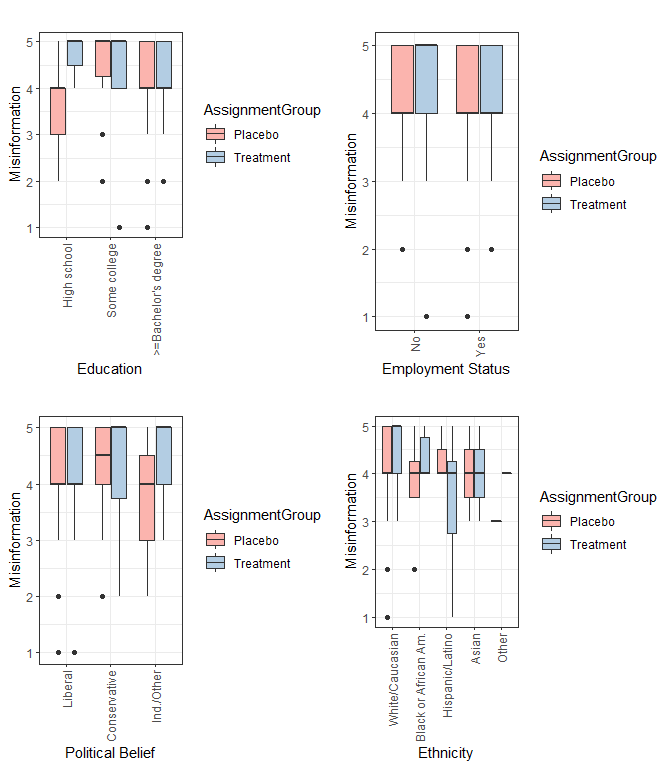
\includegraphics{FullExperiment_files/figure-latex/unnamed-chunk-51-1.pdf}

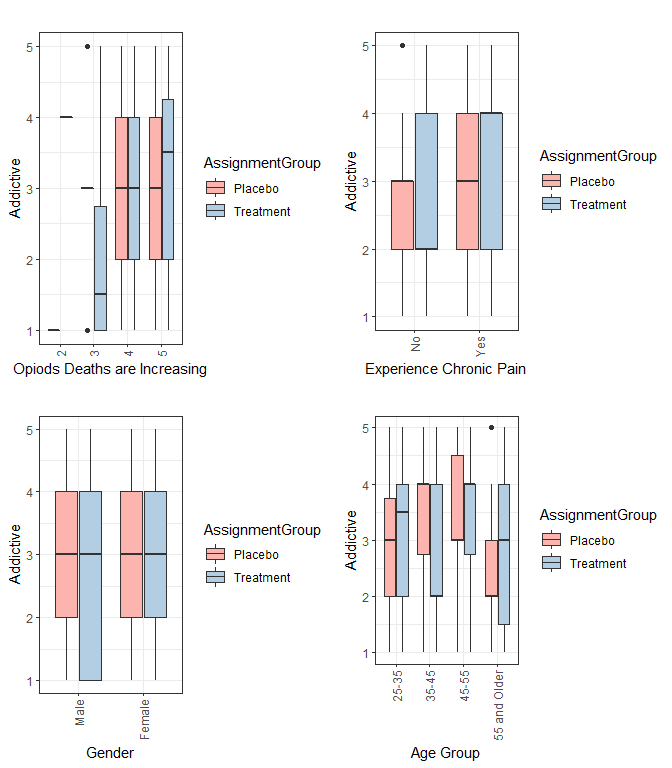
\includegraphics{FullExperiment_files/figure-latex/unnamed-chunk-52-1.pdf}

\hypertarget{medical-cannabis-is-generally-portrayed-as-more-harmful-than-it-actually-is}{%
\subsubsection{Medical cannabis is generally portrayed as more harmful
than it actually
is}\label{medical-cannabis-is-generally-portrayed-as-more-harmful-than-it-actually-is}}

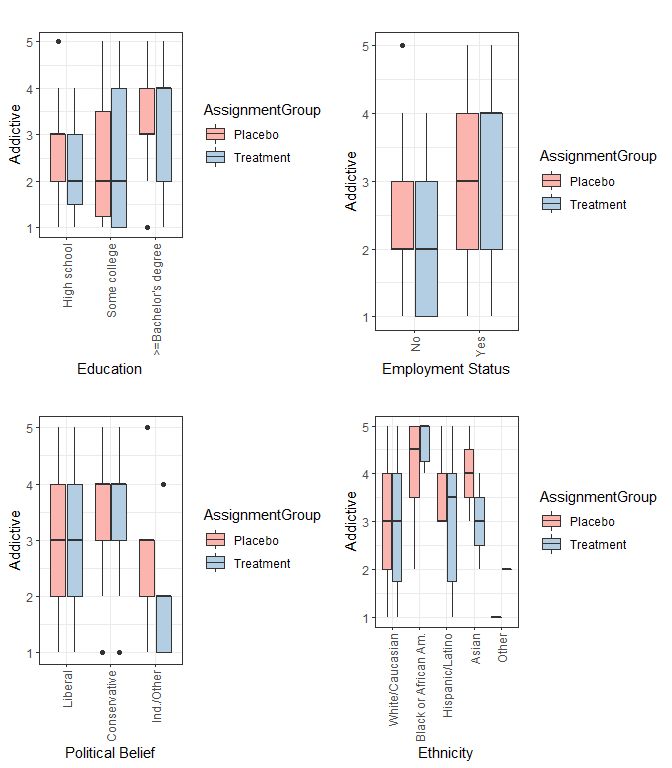
\includegraphics{FullExperiment_files/figure-latex/unnamed-chunk-53-1.pdf}

\includegraphics{FullExperiment_files/figure-latex/unnamed-chunk-54-1.pdf}

\hypertarget{there-is-a-lot-of-misinformation-about-medical-cannabis}{%
\subsubsection{There is a lot of misinformation about medical
cannabis}\label{there-is-a-lot-of-misinformation-about-medical-cannabis}}

\includegraphics{FullExperiment_files/figure-latex/unnamed-chunk-55-1.pdf}

\includegraphics{FullExperiment_files/figure-latex/unnamed-chunk-56-1.pdf}

\hypertarget{medical-cannabis-is-addictive-1}{%
\subsubsection{Medical cannabis is
addictive}\label{medical-cannabis-is-addictive-1}}

\includegraphics{FullExperiment_files/figure-latex/unnamed-chunk-57-1.pdf}

\includegraphics{FullExperiment_files/figure-latex/unnamed-chunk-58-1.pdf}

\hypertarget{user-consent}{%
\subsection{User Consent}\label{user-consent}}

We are conducting an academic survey about opinions on various
painkillers - \emph{notably opioids and medical cannabis}.

This online survey will ask you about your \emph{history with pain as
well (if you have any)}. Your participation in this online survey is
\emph{voluntary}. You may choose not to participate.

The procedure involves filling an online survey that will take
approximately 10 minutes. Your responses will be \emph{confidential} and
we do not collect information that will personally identify you.

We will do our best to keep your information confidential. All data is
stored in a password protected electronic format.

\textbf{By participating in this Survey, you are agreeing to the
following}:

\begin{enumerate}
\def\labelenumi{\arabic{enumi}.}
\tightlist
\item
  you have read the above information
\item
  you voluntarily agree to participate
\item
  you are at least 21 years of age
\end{enumerate}

If you choose to proceed, please select the link below to complete the
survey. At the end of the survey, you will receive a code to paste into
the box below to receive credit for taking our survey.

\end{document}
